%.net package
%	what are the classes provided by package and its uses
%	COnnection oriented
%		ServerSocket
%		Socket
%	Connection Less
%		Datagram Socket
%		Datagram Packet
%	Other important classes

\section{Java.net Package}
The java.net package provides a powerful and flexible infrastructure for networking. Figure \ref{netStructure} shows the class hierarchy for this package.
\begin{figure}[]
			\begin{center}
			\setlength{\unitlength}{1pt}
			\begin{picture}(453,557)(0,0)
			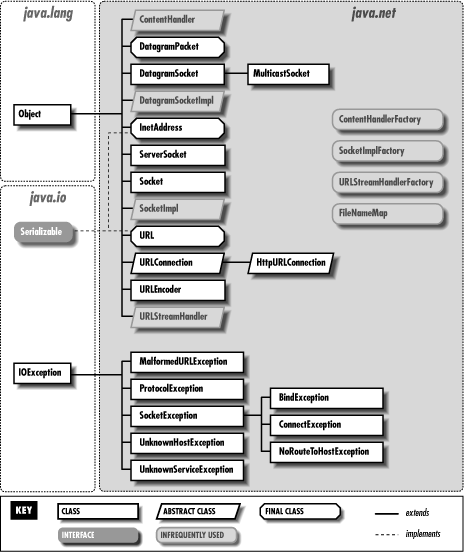
\includegraphics[width=453pt]{./NetworkingTechnologies/java/netStructure.png}
			\end{picture}
	\caption{The java.net package}
	\label{netStructure}
	\end{center}
	\end{figure}
\subsection{Classes for Connection Oriented Communication}
Connection Oriented communication is made possible by using TCP/IP protocol and classes that support socket based communication based on TCP/IP protocol. These sockets are used to implement reliable, bidirectional, persistent, point-to- point, stream-based connections between hosts on the Internet. A socket can be used to connect Java�s I/O system to other programs that may reside either on the local machine or on any other machine on the Internet. One is for servers, and the other is for clients. They are:

\begin{enumerate}
	\item \textbf{ServerSocket}\\
		Java has a different socket class that is used for crating server applications. The ServerSocket class is used to create servers that listen for local or remote client programs to connect to them on published ports. When a ServerSocket is created, it will register itself with the system as having an intrest in client connections. The constructor of ServerSocket class has the format \emph{ServerSocket(int port) throws IOException}. ServerSocket has a method called \textbf{accept()}, which is a blocking call that will wait for a client to initiate communication and then return with a normal Socket that is used for communication with client. ServerSocket class uses TCP/IP protocol for communication.
	
	\item \textbf{Socket}\\
	The Socket class is for clients and is designed to connect to ServerSocket and initiate protocol exchanges. Creation of Socket object implicitly establishes a connection between client and server. The constructor of Socket class has the following formats
	\begin{itemize}
		\item \emph{Socket(String hostName, int port) throws UnknownHostException,IOException}
		\item \emph{Socket(InetAddress ipaddress, int port) throws IOException}
	\end{itemize} 
	Input and output streams associated with a Socket can be retrieved by using \emph{getInputStream()} and \emph{getOutputStream()}.
	
\end{enumerate}

\subsection{Classes for Connection-less Communication}
TCP/IP-style networking provides predictable and serialized, reliable stream of packet data. but however using TCP/IP tends to be inefficient as it requires a dedicated connection and several other features like retransmission of lost data etc. Here Connection-less data communication provides an alternative. Connection-less communication is made possible by using UDP protocol and classes that can transport Datagrams from one machine to another without using a dedicated connection. Datagrams are bundles of information that are passed between machines. Java implements datagrams on top of UDP protocol by using two classes:
\begin{enumerate}
	\item \textbf{DatagramSocket}\\
	DatagramSocket class has four constructor formats.
	\begin{itemize}
		\item \emph{DatagramSocket() throws SocketException}
		\item \emph{DatagramSocket(int port) throws SocketException}
		\item \emph{DatagramSocket(int port, InetAddress ipAddress) throws SocketException}
		\item \emph{DatagramSocket(SocketAddress address) throws SocketException}
	\end{itemize}
	The first creates a DatagramSocket bound to any unused port on the local computer. The second creates a DatagramSocket bound to port specified by \emph{port}. The third creates a DatagramSocket bound to specified port and InetAddress while fourth constructs a DatagramSocket bound to specified SocketAddress. Two most important method defined by DatagramSocket class are \textbf{send()} and \textbf{receive()}. send() method sends packet to the port specified by \emph{packet} while receive() method waits for a packet to be received from the port specified by \emph{packet}.
	
	\begin{itemize}	
		\item[ ] \emph{void send(DatagramPacket packet) throws IOException}
		\item[ ] \emph{void receive(DatagramPacket packet) throws IOException}
	\end{itemize}
	
	\item \textbf{DatagramPacket}\\
	Datagram Packet represents the packets which are used to send information between systems. These packets can store information as binary array. DatagramPackets constructed to send information contains the receiver address represented by InetAddress class. DatagramPacket defines several constructors.
	\begin{itemize}	
		\item \emph{DatagramPacket(byte data[ ], int size)}
		\item \emph{DatagramPacket(byte data[ ], int offset, int size)}
		\item \emph{DatagramPacket(byte data[ ], int size, InetAddress ipAddress, int port)}
		\item \emph{DatagramPacket(byte data[ ], int offset, int size, InetAddress ipAddress, int port)}
	\end{itemize}
	The first constructor specifies a buffer that will receive data, and the size of a packet. It is used for receiving data over a DatagramSocket. The second form allows you to specify an offset into the buffer at which data will be stored. The third form specifies a target address and port, which are used by a DatagramSocket to determine where the data in the packet will be sent. The fourth form transmits packets beginning at the specified offset into the data. 
\end{enumerate}

\subsection{Other Important Classes in java.net package}
\begin{enumerate}
	\item \textbf{InetAddress}\\
	The InetAddress class represents an Internet Protocol (IP) address and can be used when creating DatagramPacket or Socket objects. The class does not have public constructor functions. Instead it supports three static methods which return one or more instances of InetAddress. The InetAddress class contains two fields namely, hostName (of type String object) and address (of type int) which are not public. The hostName field contains the name of host and the address field contains the 32 bit IP address, for e.g.. 140.105.16.63 (this is IPv4. This representation will be different for a 16 byte IPv6 address). The \emph{getLocalHost()}, \emph{getByName()} and \emph{getAllByName()} methods must be used by applications to create a new InetAddress instance. The syntax of these methods are as folllows:
	\begin{itemize}
		\item[ ] \emph{public static InetAddress getLocalHost()throws UnknownHostException}
		\item[ ] \emph{public static InetAddress getByName(String host)throws UnknownHostException}
		\item[ ] \emph{public static InetAddress[] getAllByName(String host)throws UnknownHostException}
	\end{itemize}
	
%	\item \textbf{URL}\\
%	Class URL represents a Uniform Resource Locator, a pointer to a "resource" on the World Wide Web. A resource can be something as simple as a file or a directory, or it can be a reference to a more complicated object, such as a query to a database or to a search engine. 
\end{enumerate}